\chapter{Priprava na 10. laboratorijske vaje}
\section{Realizacija končnih avtomatov s pomnilnimi celicami (Moorov avtomat)}

Z uporabo logičnih vrat in pomnilnih celic želimo realizirati Moorov avtomat. Postopek realizacije je sestavljen iz sledečih korakov:
\begin{enumerate}
\item \emph{Zapis kodirnih tabel}: vhodna abeceda, notranja abeceda in izhodna abeceda so predstavljene z abstraktnim zapisom. Za realizacijo s preklopnimi funkcijami moramo le-te predstaviti s preklopnimi spremenljivkami. Pri tem upoštevamo dejstvo, da lahko z $i$ vhodnimi spremenljivkami zakodiramo $2^i$ vhodnih črk, z $j$ izhodnimi spremenljivkami $2^j$ izhodnih črk, s $k$ pomnilnimi celicami pa $2^k$ notranjih stanj. S kodiranimi tabelami povežemo posamezne spremenljivke oziroma notranja stanja pomnilnih celic s posameznimi črkami oziroma stanji avtomata.
\item \emph{Zapis pravilnostne tabele avtomata}: na podlagi diagrama prehajanja stanj oziroma tabele prehajanja stanj in kodirnih tabel, lahko zapišemo pravilnostno tabelo avtomata. Pri tem na levi strani tabele nastopajo spremenljivke, ki določajo vhodne črke in trenutna notranja stanja avtomata (neodvisne spremenljivke), na desni strani pa spremenljivke, ki določajo notranje stanje avtomata v naslednjem časovnem koraku in spremenljivke, ki določajo izhodne črke avtomata (odvisne spremenljivke).
\item \emph{Določitev vhodov v pomnilne celice}: na podlagi prehodov med spremenljivkami, ki določajo trenutno stanje avtomata in stanje avtomata v naslednjem časovnem koraku ter vzbujevalnih tabel pomnilnih celic, ki jih imamo na razpolago, lahko določimo potrebne vhode v pomnilne celice v posamezni vrstici (tabelo dopolnimo na podoben način kot smo jo pri realizaciji sekvenčnih vezij s pomnilnimi celicami). 
\item \emph{Izpis in minimizacija izhodne funkcije in funkcije prehajanja stanj}: na podlagi pravilnostne tabele lahko s pomočjo Veitchevega diagrama izpišemo preklopne funkcije, ki določajo izhodne črke avtomata (izhodna funkcija) in preklopne funkcije, ki nastopajo na vhodih pomnilnih celic in tako določajo prehode med stanji avtomata (funkcija prehajanja stanj)
\end{enumerate}

\bigskip

\begin{zgled}

Z uporabo T pomnilnih celic in poljubnih logičnih vrat realiziraj Moorov avtomat, ki je podan z diagramom prehajanja stanj.

%\begin{center}
%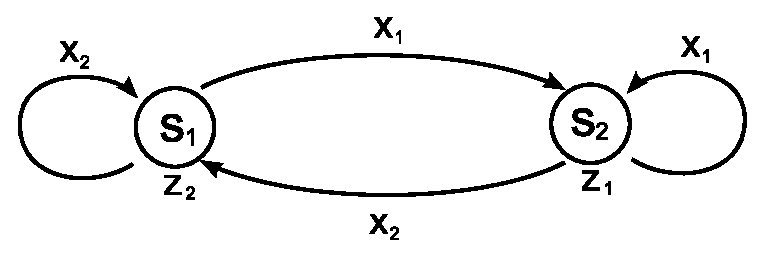
\includegraphics[width=0.5\linewidth]{slika_v10_1.eps}
%\end{center}

\begin{center}
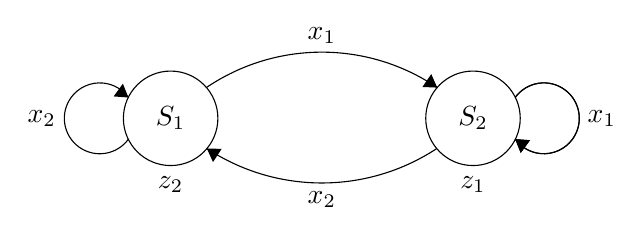
\begin{tikzpicture}[scale=0.2]
\tikzstyle{every node}+=[inner sep=0pt]
%\node[draw] at (0,0) {some text};
\draw [black] (20.5,-17.8) circle (3);
\draw (20.5,-17.8) node {$S_1$};
\draw (20.5,-22) node {$z_2$};
\draw [black] (39.7,-17.8) circle (3);
\draw (39.7,-17.8) node {$S_2$};
\draw (39.7,-22) node {$z_1$};
\draw [black] (22.769,-15.848) arc (124.12588:55.87412:13.067);
\fill [black] (37.43,-15.85) -- (37.05,-14.99) -- (36.49,-15.81);
\draw (30.1,-13.1) node [above] {$x_1$};
\draw [black] (37.402,-19.718) arc (-56.63019:-123.36981:13.275);
\fill [black] (22.8,-19.72) -- (23.19,-20.58) -- (23.74,-19.74);
\draw (30.1,-22.41) node [below] {$x_2$};
\draw [black] (17.82,-19.123) arc (-36:-324:2.25);
\draw (13.25,-17.8) node [left] {$x_2$};
\fill [black] (17.82,-16.48) -- (17.47,-15.6) -- (16.88,-16.41);
\draw [black] (42.38,-16.477) arc (144:-144:2.25);
\draw (46.95,-17.8) node [right] {$x_1$};
\fill [black] (42.38,-19.12) -- (42.73,-20) -- (43.32,-19.19);
\draw [black] (42.38,-16.477) arc (144:-144:2.25);
\fill [black] (42.38,-19.12) -- (42.73,-20) -- (43.32,-19.19);
\end{tikzpicture}
\end{center}

\end{zgled}

\begin{resitev}

Postopek je sledeč:

\begin{enumerate} 

\item Zapišemo kodirne tabele, ki določijo kodiranje vhodne abecede, notranje abecede in izhodne abecede. Za zapis vseh črk vhodne abecede je dovolj ena vhodna spremenljivka ($x$); prav tako je za zapis vseh črk izhodne abecede dovolj ena izhodna spremenljivka ($y$). Ker imamo zgolj dve notranji stanji avtomata, je za njegovo realizacijo potrebna ena pomnilna celica T z notranjim stanjem $q$. Kodirne tabele so torej

\begin{table}[ht]
\begin{center}
\begin{tabular}{ccc}
	\begin{tabular}{c|c}
	 & $x$ \\ 
		\hline
		$x_1$ & $0$\\
		$x_2$ & $1$\\
	\end{tabular}
	&
	\begin{tabular}{c|c}
		 & $q$ \\ 
		\hline
		$S_1$ & $0$\\
		$S_2$ & $1$\\
	\end{tabular}
	&
	\begin{tabular}{c|c}
		 & $y$ \\ 
		\hline
		$z_1$ & $0$\\
		$z_2$ & $1$\\
	\end{tabular}
\end{tabular}
\end{center}
\end{table}

\bigskip

\item Na podlagi kodirnih tabel in podanega diagrama prehajanja stanj lahko zapišemo pravilnostno tabelo avtomata. Pri tem na levi strani tabele nastopajo spremenljivke, ki določajo trenutno notranje stanje avtomata ($q$) in vhodno črko ($x$), na desni pa spremenljivke, ki določajo notranje stanje avtomata v naslednjem časovnem koraku ($D^1q$) in izhodno črko ($y$):

\begin{center}
\begin{tabular}{cc|cc}
 $q$ & $x$ & $D^1 q$ & $y$\\
 \hline
 0 & 0 & 1 & 1\\		 
 0 & 1 & 0 & 1\\
 1 & 0 & 1 & 0\\
 1 & 1 & 0 & 0\\
\end{tabular}
\end{center}

\bigskip

\item Na podlagi prehodov med spremenljivkami $q$ in $D^1q$ in vzbujevalne tabele za T pomnilno celico, lahko določimo vrednosti, ki morajo biti na vhodu $t$ pri posamezni kombinaciji vhodnih spremenljivk:

\begin{center}
\begin{tabular}{cc|cc|c}
 $q$ & $x$ & $D^1 q$ & $y$ & $t$\\
 \hline
 0 & 0 & 1 & 1 & 1 \\		 
 0 & 1 & 0 & 1 & 0 \\
 1 & 0 & 1 & 0 & 0 \\
 1 & 1 & 0 & 0 & 1 \\
\end{tabular}
\end{center}

\bigskip

\item Na podlagi pravilnostne tabele lahko s pomočjo Veitchevega diagrama izpišemo funkcijo, ki nastopa na vhodu T pomnilne celice in izhodno funkcijo avtomata:


\begin{figure}[!ht]
\begin{center}
\begin{tabular}{cc}
\includegraphics{veitch_moore_t.eps} &
\includegraphics{veitch_moore_y.eps} \\
$t = \ol x\ \ol q \vee x q = x \equiv q$ & $y = \ol q$\\
\end{tabular}
\end{center}
\end{figure}


Če funkcijo na vhodu T pomnilne celice vstavimo v enačbo T pomnilne celice ($D^1 q = t \ol q \vee \ol t q$), dobimo \emph{funkcijo prehajanja stanj} avtomata:
$$
D^1q = (x \equiv q) \ol q \vee \ol{(x \equiv q)} q = (x \equiv q) \ol q \vee (x \nabla q) q 
$$ 

Po definiciji velja, da je izhodna črka Moorovega avtomata določena s trenutnim stanjem avtomata. Velja torej, da je izhodno črko pri Moorovem avtomatu vedno mogoče izraziti zgolj s spremenljivkami, ki določajo trenutno stanje avtomata (v našem primeru $y=\ol q$).

\end{enumerate}

\bigskip

Realizacijo avtomata v Logisimu prikazuje slika \ref{fig:logisim1}.


\begin{figure}[ht]
\begin{center}
\includegraphics[width=0.75\linewidth]{moore_logisim_1.eps}
\end{center}
\caption{Realizacija avtomata iz zgleda v Logisimu.}
\label{fig:logisim1}
\end{figure}

\end{resitev}

\newpage

\begin{zgled}

Z uporabo D pomnilnih celic realiziraj Moorov avtomat, podan s tabelo

\begin{center}
\begin{tabular}{c|ccc}
& $z_1$ & $z_2$ & $z_3$\\
& $S_1$ & $S_2$ & $S_3$\\
\hline
$x_1$ & $S_1$ & $S_1$ & $S_1$\\
$x_2$ & $S_2$ & $S_3$ & $S_2$\\
\end{tabular}
\end{center}

\end{zgled}

\begin{resitev}
Postopek je sledeč:

\begin{enumerate} 
\item Za zapis dveh črk vhodne abecede je dovolj ena vhodna spremenljivka ($x$). Ker ima izhodna abeceda tri črke, za njen zapis potrebujemo dve spremenljivki ($y_1$ in $y_2$). Ker imamo tri notranja stanja avtomata, sta za njegovo realizacijo potrebni dve pomnilni celici D z notranjimi stanji $q_1$ in $q_2$. Kodirne tabele so torej

\begin{table}[ht]
\begin{center}
\begin{tabular}{ccc}
\begin{tabular}{c|c}
& $x$\\
\hline
$x_1$ & $0$\\
$x_2$ & $1$
\end{tabular}
&
\begin{tabular}{c|cc}
& $q_1$ & $q_2$\\
\hline
$S_1$ & $0$ & $0$\\
$S_2$ & $0$ & $1$\\
$S_3$ & $1$ & $0$
\end{tabular}
&
\begin{tabular}{c|cc}
& $y_1$ & $y_2$\\
\hline
$z_1$ & $0$ & $0$\\
$z_2$ & $0$ & $1$\\
$z_3$ & $1$ & $0$
\end{tabular}
\end{tabular}
\end{center}
\end{table}

\bigskip

\item Zapišemo pravilnostno tabelo avtomata (ko je $q_1=1$ in $q_2=1$, funkcijska vrednost ni določena):

\begin{center}
\begin{tabular}{ccc|cccc}
$q_1$ & $q_2$ & $x$ & $D^1 g_1$ & $D^1 g_2$ & $y_1$ & $y_2$\\
\hline
0 & 0 & 0 & 0 & 0 & 0 & 0\\
0 & 0 & 1 & 0 & 1 & 0 & 0\\
0 & 1 & 0 & 0 & 0 & 0 & 1\\
0 & 1 & 1 & 1 & 0 & 0 & 1\\
1 & 0 & 0 & 0 & 0 & 1 & 0\\
1 & 0 & 1 & 0 & 1 & 1 & 0\\
1 & 1 & 0 & ? & ? & ? & ?\\
1 & 1 & 1 & ? & ? & ? & ?\\
\end{tabular}
\end{center}

\bigskip

\item Na podlagi prehodov iz spremenljivke $q_1$ v $D^1q_1$ ter prehodov iz spremenljivke $q_2$ v $D^1q_2$, lahko določimo vrednosti, ki morajo biti na vhodu D pomnilnih celic (pomnilna celica z vhodom $d_1$ bo hranila notranje stanje $q_1$, celica z vhodom $d_2$ pa $q_2$):

\begin{center}
\begin{tabular}{ccc|cccc|cc}
$q_1$ & $q_2$ & $x$ & $D^1 g_1$ & $D^1 g_2$ & $y_1$ & $y_2$ & $d_1$ & $d_2$\\
\hline
0 & 0 & 0 & 0 & 0 & 0 & 0 & 0 & 0\\
0 & 0 & 1 & 0 & 1 & 0 & 0 & 0 & 1\\
0 & 1 & 0 & 0 & 0 & 0 & 1 & 0 & 0\\
0 & 1 & 1 & 1 & 0 & 0 & 1 & 1 & 0\\
1 & 0 & 0 & 0 & 0 & 1 & 0 & 0 & 0\\
1 & 0 & 1 & 0 & 1 & 1 & 0 & 0 & 1\\
1 & 1 & 0 & ? & ? & ? & ? & ? & ?\\
1 & 1 & 1 & ? & ? & ? & ? & ? & ?\\
\end{tabular}
\end{center}

\bigskip

\item Določimo funkcije za realizacijo:


\begin{figure}[!ht]
\begin{center}
\begin{tabular}{cc}
\includegraphics{veitch_moore_d_1.eps} &
\includegraphics{veitch_moore_d_2.eps} \\
$d_1 = q_2 x$ & $d_2 = \ol q_2 x$\\
\end{tabular}
\end{center}
\end{figure}

\begin{figure}[!ht]
\begin{center}
\begin{tabular}{cc}
\includegraphics{veitch_moore_y_1.eps} &
\includegraphics{veitch_moore_y_2.eps} \\
$y_1 = q_1$ & $y_2 = q_2$\\
\end{tabular}
\end{center}
\end{figure}

\bigskip



Realizacijo avtomata v Logisimu prikazujejo slike \ref{fig:logisim2}, \ref{fig:logisim2_d}(a) in \ref{fig:logisim2_d}(b).

\begin{figure}[ht]
\begin{center}
\includegraphics[width=0.75\linewidth]{moore_logisim_2.eps}
\end{center}
\caption{Realizacija avtomata iz zgleda v Logisimu. Zaradi splošnosti sheme sta funkciji, ki vstopata v pomnilni celici D, umeščeni v ločena modula (glej sliki \ref{fig:logisim2_d}(a) in \ref{fig:logisim2_d}(b)).}
\label{fig:logisim2}
\end{figure}


\begin{figure}[!ht]
\begin{center}
\begin{tabular}{cc}
\includegraphics[width=0.4\linewidth]{moore_logisim_2_d1.eps} &
\includegraphics[width=0.4\linewidth]{moore_logisim_2_d2.eps} \\
(a) & (b) \\
\end{tabular}
\caption{Realizacija preklopne funkcije, ki vstopa v D pomnilno celico z vhodom $d_1$ (a) in preklopne funkcije, ki vstopa v D pomnilno celico z vhodom $d_2$ (b).}
\label{fig:logisim2_d}
\end{center}
\end{figure}

%\bigskip
%Funkcija prehajanja stanj:\\
%$t_1(g_1, g_2, x) = g_1 \vee g_2 x$\\
%$t_2(g_1, g_2, x) = q_2 \vee x$

%\bigskip
%Izhodna funkcija:\\
%$y_1(q_1, q_2) = q_1$\\
%$y_2(q_1, q_2) = q_2$

\end{enumerate}
\end{resitev}